\documentclass[fleqn]{beamer}
\usepackage[english]{babel}

\usepackage{amsmath,amssymb}
\usepackage{graphicx}
\usepackage{multicol}
\usepackage{hyperref}

% vertical separator macro
\newcommand{\vsep}{
  \column{0.0\textwidth}
    \begin{tikzpicture}
      \draw[very thick,black!10] (0,0) -- (0,7.3);
    \end{tikzpicture}
}

\newcommand{\quotes}[1]{``#1''}

\newcommand{\drawkey}[1]{%
  \begingroup\normalfont
  \includegraphics[scale=.3]{setup_guide//keys/#1.png}%
  \endgroup
}

% More space between lines in align
\setlength{\mathindent}{0pt}
% double spacing in paragraphs
\setlength{\parskip}{1em}

% Beamer theme
\usetheme{ZMBZFMK}
\usefonttheme[onlysmall]{structurebold}
\mode<presentation>
%\setbeamercovered{transparent=10}

% align spacing
\setlength{\jot}{0pt}

% Uncomment if you wish to use a TOC

% \AtBeginSection[]
% {
%   \begin{frame}
%     \frametitle{Table of Contents}
%     \tableofcontents[currentsection]
%   \end{frame}
% }
% \AtBeginSubsection[]
% {
%   \begin{frame}
%     \frametitle{Table of Contents}
%     \tableofcontents[currentsubsection]
%   \end{frame}
% }


% Only the first Slide
\title{Quartus/Questa Install Guide}
\author{Rich Baird}
\institute[University of Utah]{}
\date{\today}


% Title
\begin{document}
\begin{frame}
  \titlepage
\end{frame}

% Frame 1
\section{Questa Installation Guide}
\begin{frame}
  \frametitle{Motivation}
    Starting with Intel® Quartus® Prime version 21.3, the ModelSim*-Intel® FPGA edition software has been discontinued and replaced by the Questa*-Intel® FPGA. This change has since made its way to the lite edition in 21.1. \par
    Overall this is a welcome update as Modelsim has not been in active development for some time. However, the installation and licensing process can be a bit of a challenge. This guide will take you through the process of installing and setting up Questa so that you may begin writing and running your simulations.
\end{frame}

\subsection{Obtaining the software}
\begin{frame}{Software Installation}
    To begin, navigate in your preferred browser to \url{https://fpgasoftware.intel.com}. You will be directed to a website with links to download various software. Select Quartus Prime Lite.
    
\begin{figure}
    \centering
    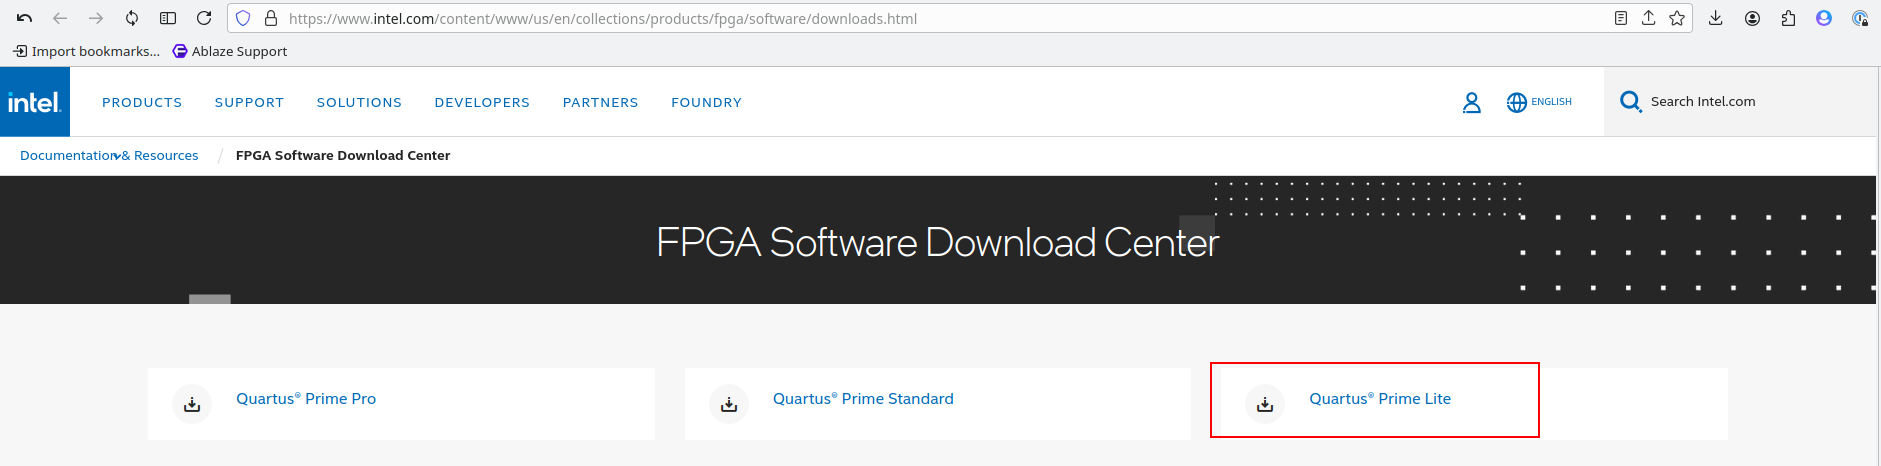
\includegraphics[width=1\linewidth]{setup_guide//figures/qprimelite_download.png}
    \caption{Select the Quartus Prime Lite download link}
    \label{fig:qprime_dl}
\end{figure}
\end{frame}

\begin{frame}{Software Installation}
    On the next page, under the Downloads section, choose to download the automated installer.
    \begin{figure}
        \centering
        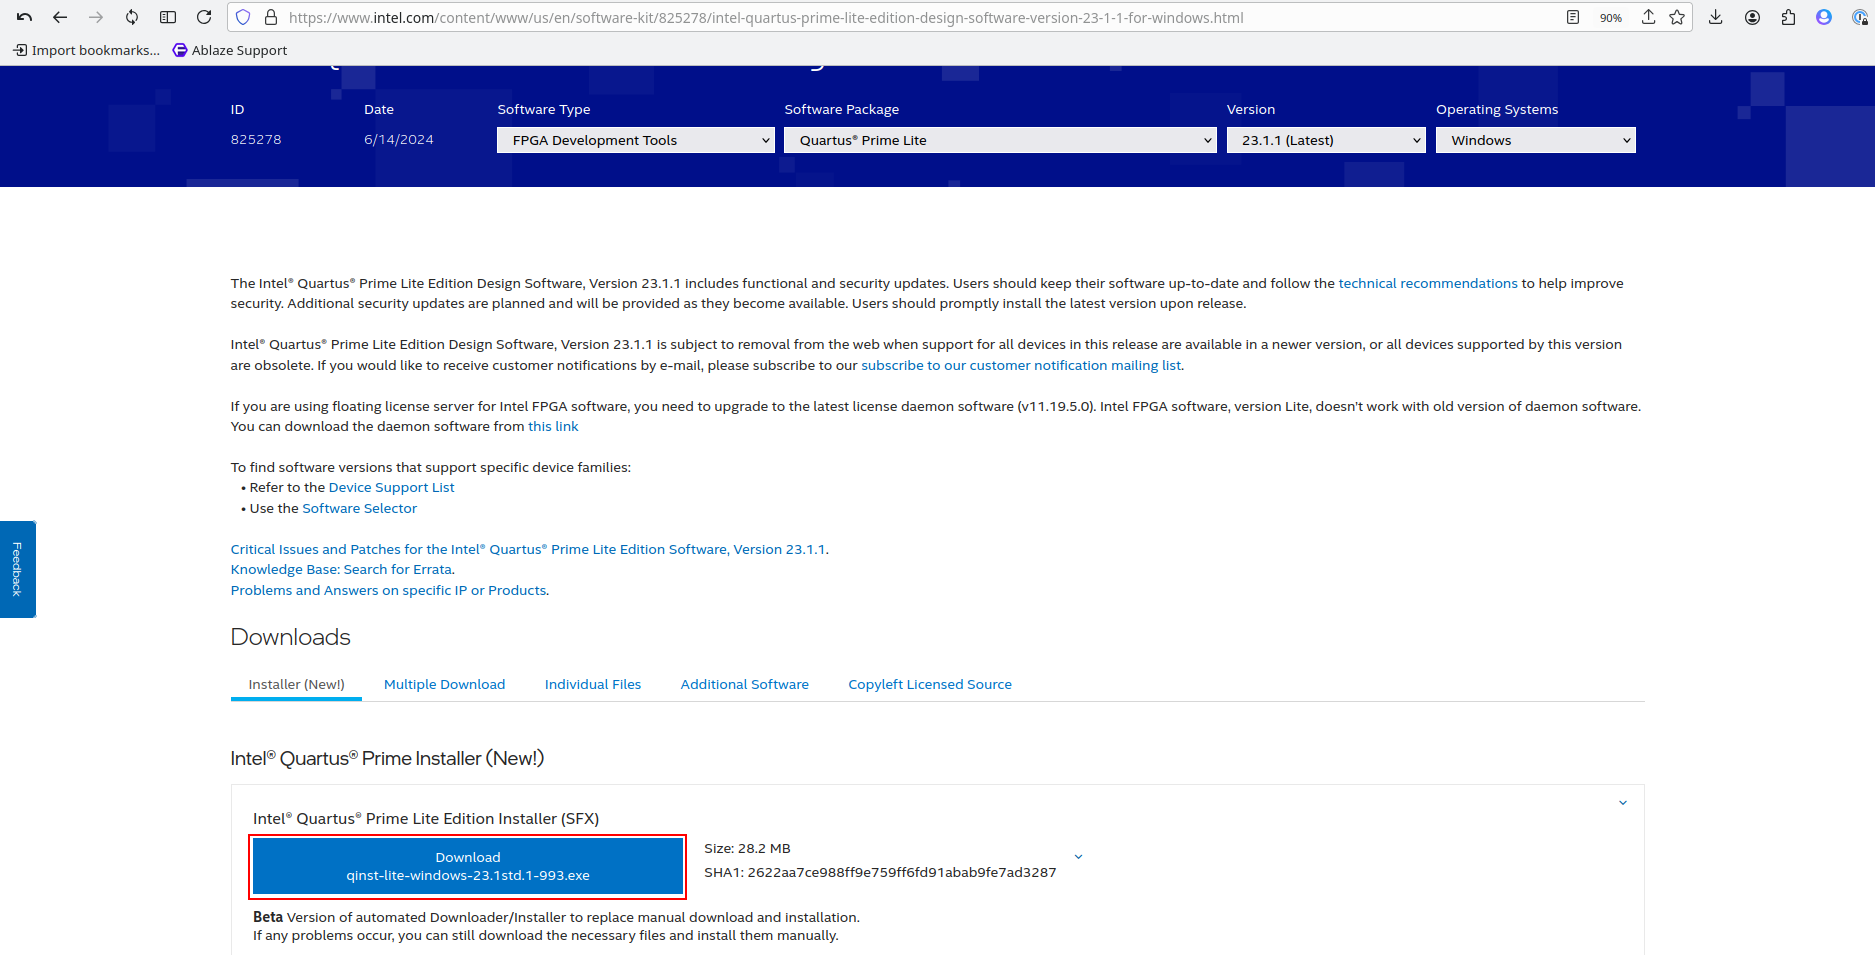
\includegraphics[width=1\linewidth]{setup_guide//figures/auto_installer.png}
        \caption{Download the automated installer}
        \label{fig:enter-label}
    \end{figure}
\end{frame}
\subsection{Installing the software}
\begin{frame}{Software Installation}
    Once the download is complete, run the installer. You will see a screen with multiple options. Ensure the following items are selected and then press Download. The download may take some time.
    \begin{itemize}
        \item Quartus Prime Lite Edition (Free) and all sub-items
        \item Devices: Max 10 FPGA Device Support
        \item Auto install after download
        \item Agree to intel license agreement
        \item After install actions
    \end{itemize}
    See the figure on the next page
\end{frame}
\begin{frame}{Software Installation}
        \begin{figure}
        \centering
        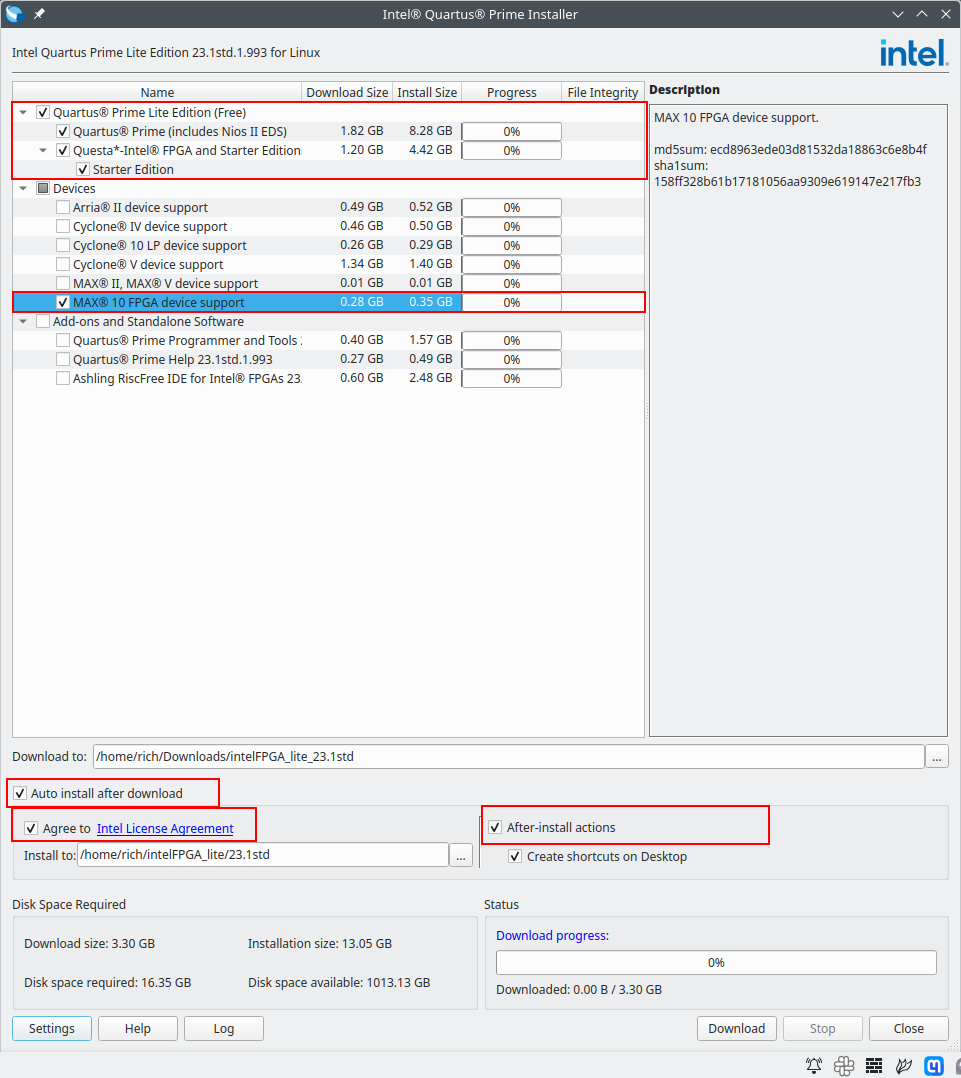
\includegraphics[width=\textwidth,height=\textheight,keepaspectratio]{setup_guide//figures/installer_1.png}
        \caption{Make sure you have selected Questa and Max 10 options}
        \label{fig:enter-label}
    \end{figure}
\end{frame}
\subsection{Obtaining a license}
\begin{frame}{Get a license}
    While the download is in progress, use this time to obtain a free license to use the new software. This can be obtained by navigating in your preferred browser to \url{https://licensing.intel.com/}. You will have the option to sign-in or enroll. Choose enroll to create a new account. Follow the steps in the form to create a new account. \textbf{Use an email other than your school email. Using your school email will cause the licensing portal to attempt to log in via Azure, which will not work.} Once complete, the enrollment process is performed automatically and may take up to 30 minutes. You will receive an email when your account is ready.
\end{frame}
\begin{frame}{Get a license}
    Once you have completed the registration and are able to log into the licensing site, from the menu select \quotes{Sign up for Evaluation or Free Licenses}. From that page, select the 2nd option in the table \quotes{Questa*-Intel® FPGA Starter Edition} and set the \# of seats to 1.
    \begin{multicols}{2}
        \begin{figure}
            \centering
            
\includegraphics[scale=.3]{figures/freelicenses.png}
            \caption{Sign up for Free Licenses}
            \label{fig:my_label}
        \end{figure}
        \begin{figure}
            \centering
            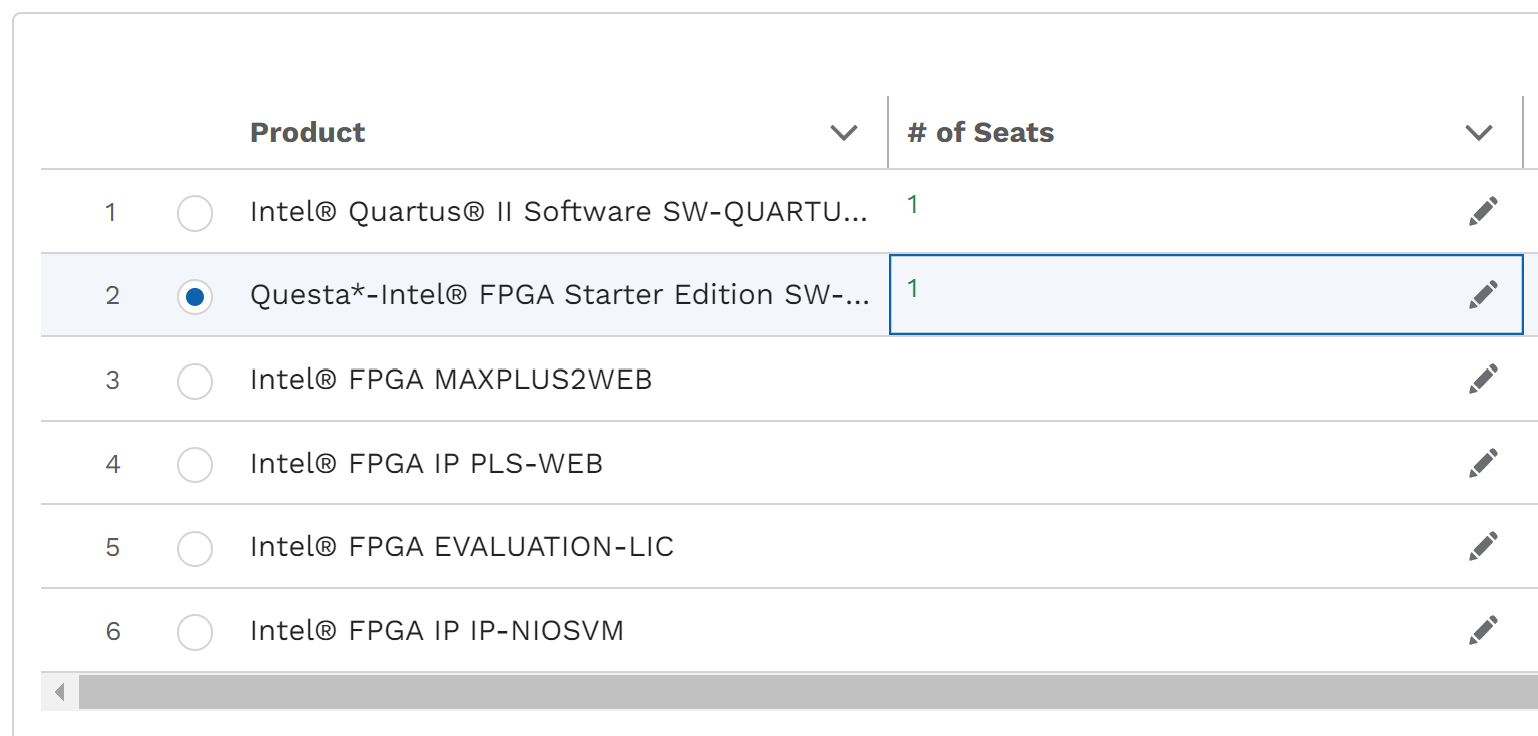
\includegraphics[scale=.3,trim={0 3cm 3cm 0},clip]{figures/questalicense.png}
            \caption{Questa License with 1 seat}
            \label{fig:my_label}
        \end{figure}
    \end{multicols}
    \vspace{-.5cm}
    Finally, mark the 2 option boxes at the bottom of the screen and press the blue \quotes{Get a License} button.
\end{frame}
\begin{frame}{Create a computer}
    In the new screen that appears, select the \quotes{+New Computer} option. Here you will need the following information \begin{itemize}
        \item Computer Name
        \item Physical NIC Address
    \end{itemize}
To obtain the first, from the launch bar of your PC, search for \quotes{This PC}. On the right side of the menu, select properties.
\vspace{-1cm}
\begin{figure}
    \centering
    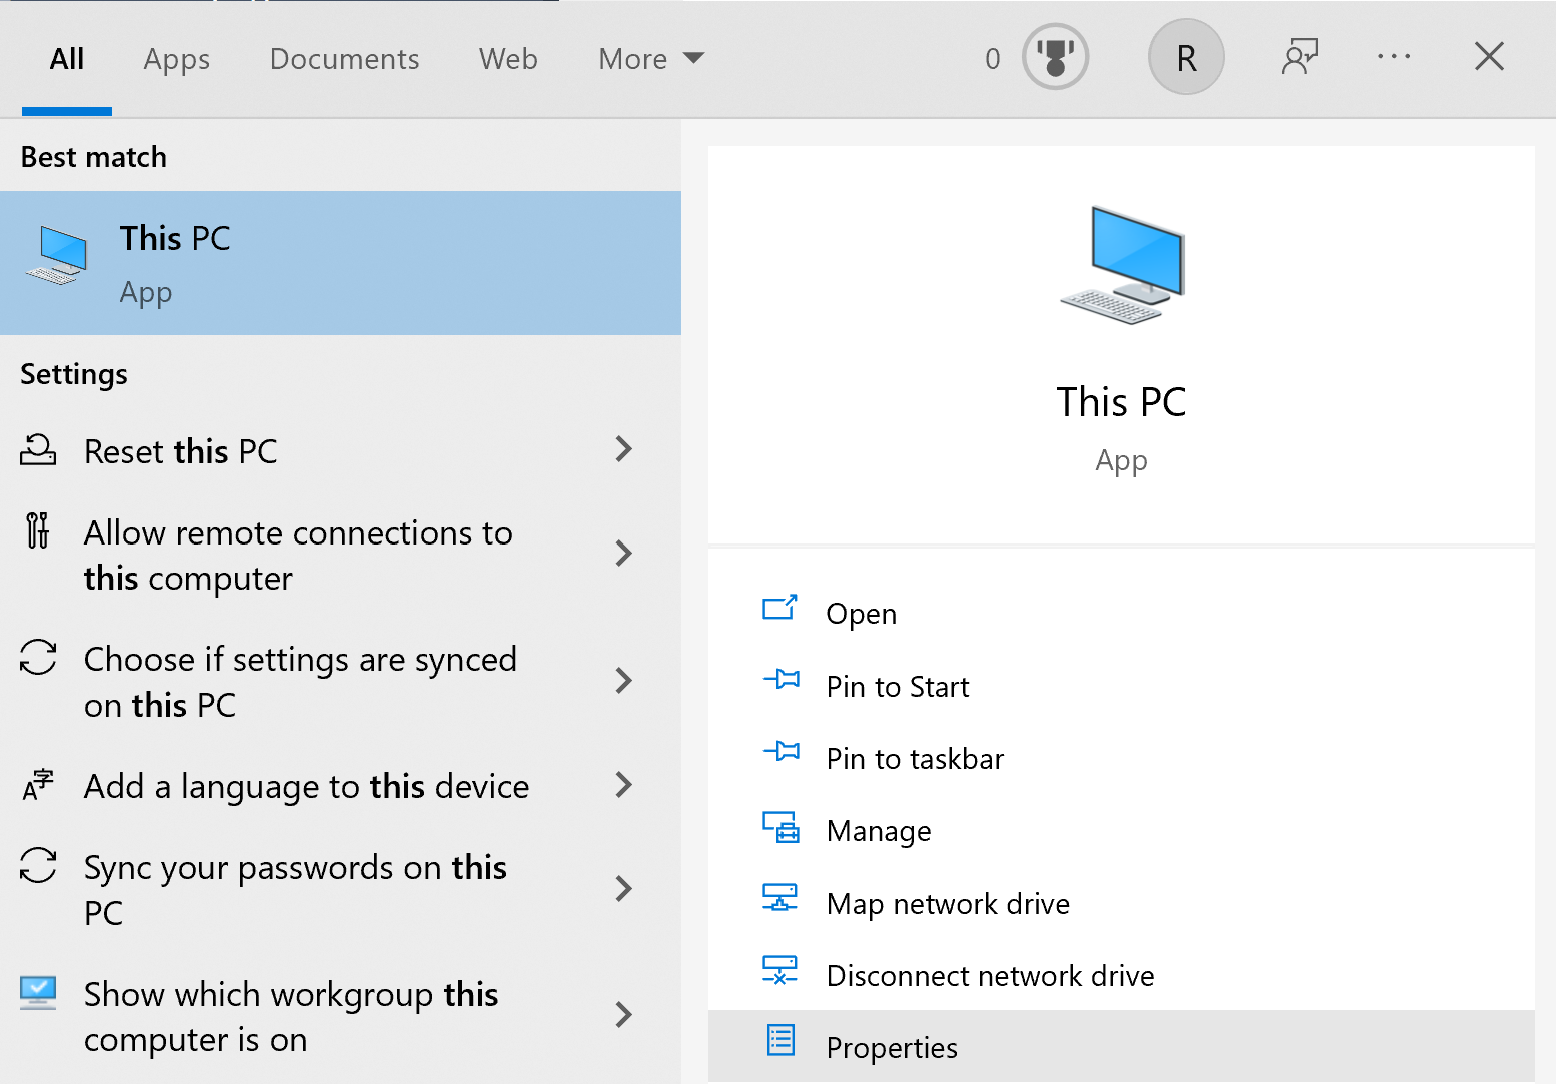
\includegraphics[scale=.2]{figures/pcproperties.png}
    \caption{Select Properties from the \quotes{This PC} menu}
    \label{fig:my_label}
\end{figure}
\end{frame}
\begin{frame}{Create a computer}
    In the properties dialog, you will find the device name under Device Specifications. Place this value in the \quotes{Computer Name} field of the Create Computer dialog on the licensing page.
    \begin{multicols}{2}
        \begin{figure}
            \centering
            
\includegraphics[scale=.4]{figures/devicename.png}
            \caption{Device name from computer properties}
            \label{fig:my_label}
        \end{figure}
        \begin{figure}
            \centering
            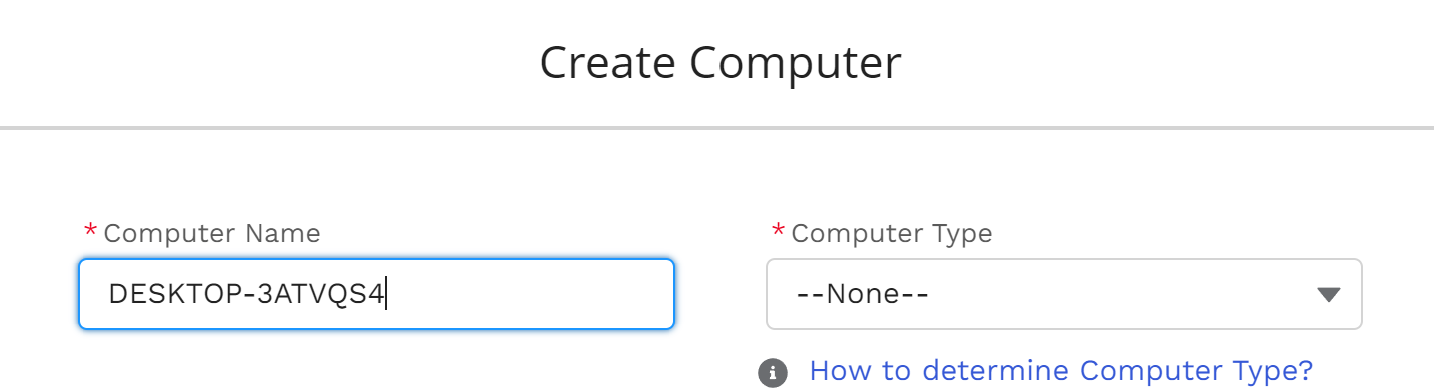
\includegraphics[scale=.3]{figures/ccmenucpuname.png}
            \caption{Create Computer Dialog}
            \label{fig:my_label}
        \end{figure}
    \end{multicols}
    Leave the properties dialog open. We will need it again later.
\end{frame}
\begin{frame}{Create a Computer}
    To obtain the physical NIC address, press \drawkey{win} + \drawkey{R} to open the run prompt. Inside the prompt type \quotes{cmd} without quotes and press OK to open the command prompt. In the command prompt that follows, type \quotes{ipconfig /all} and press enter.
    \begin{multicols}{2}
        \begin{figure}
            \centering
            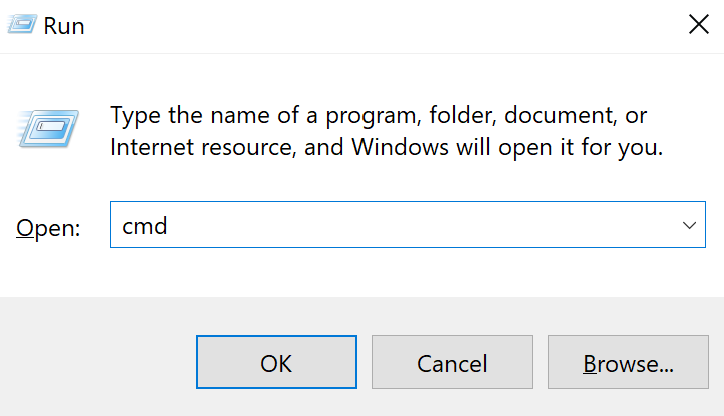
\includegraphics[scale=.5]{figures/runcmd.png}
            \caption{Run Prompt}
            \label{fig:my_label}
        \end{figure}
        \begin{figure}
            \centering
            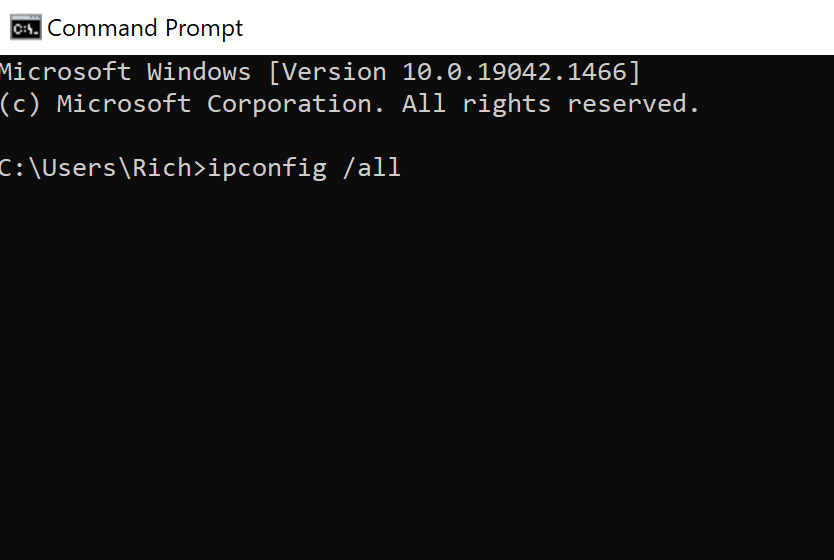
\includegraphics[scale=.5]{figures/cmd.png}
            \caption{Command prompt}
            \label{fig:my_label}
        \end{figure}
    \end{multicols}
\end{frame}
\begin{frame}{Create a Computer}
    This command will list several characteristics of your network interfaces. From this list, find the \quotes{physical address} line. Type the corresponding number without hyphens (\quotes{-}) into the Primary Computer ID field of the Create a Computer dialog. If you have multiple NICs, the dialog provides options for secondary and tertiary IDs that you can place them in. Please be aware that if you are using a virtual machine, you will need to make sure that your setup does not reinitialize mac addresses at every boot. The details of this setup are beyond the scope of this guide.
    \begin{multicols*}{2}
        \begin{figure}
            \centering
            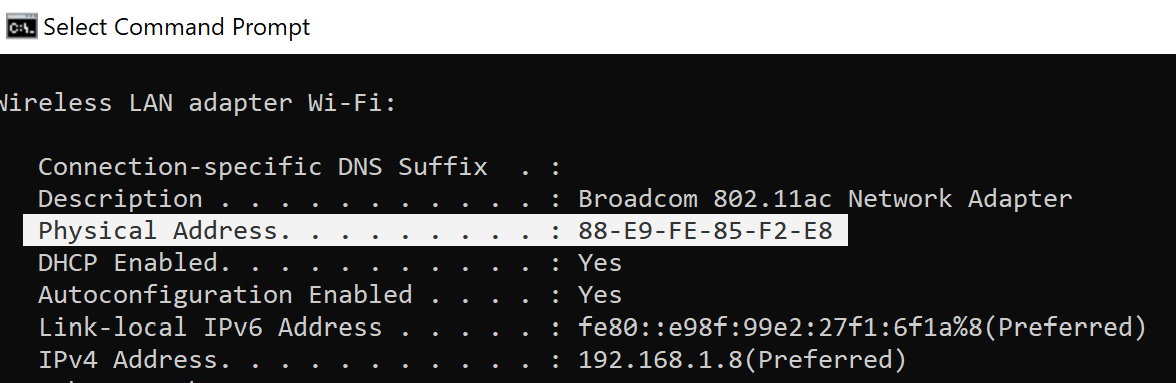
\includegraphics[scale=.3]{figures/ipconfigall.png}
            \caption{Caption}
            \label{fig:my_label}
        \end{figure}
        \begin{figure}[hbtp]
            \vspace{-1cm}
            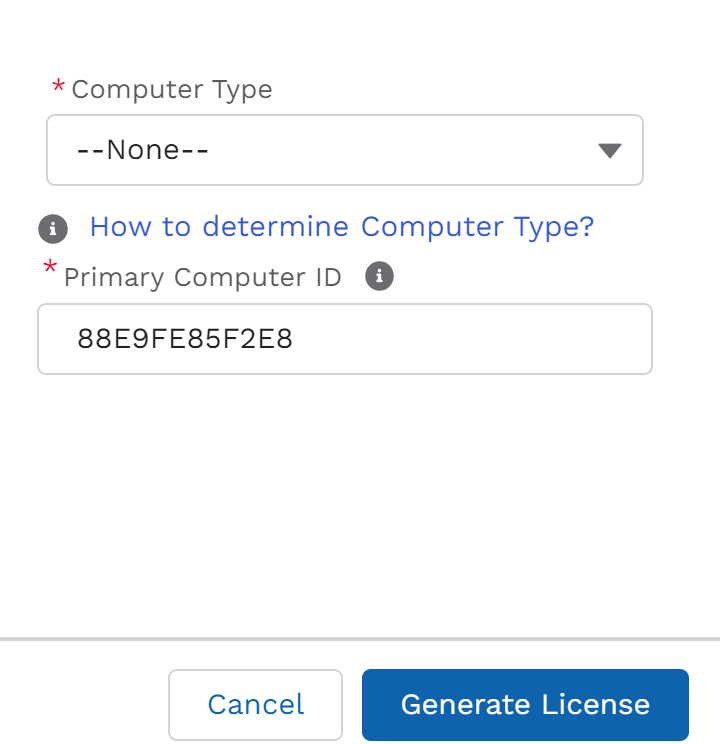
\includegraphics[scale=.6,trim={0 4cm 0 0},clip]{figures/pcid.png}
            \caption{Primary Computer ID should be the physical address}
            \label{fig:my_label}
        \end{figure}
    \end{multicols*}
\end{frame}
\begin{frame}{Create a Computer}
    Finally in the Create a Computer dialog select \quotes{License Type} and set it to fixed, and select \quotes{Primary ID} and set it to NIC. Then click on the blue \quotes{Generate License} button.
\end{frame}
\subsection{Complete Installation}
\begin{frame}{Software Installation}
    Wait for the software installation to complete before continuing.
\end{frame}
\subsection{Installing the license}
\begin{frame}{License Installation}
    Once the software is installed, download the .dat license file sent to the email associated with your login and save it to a location where it won't get accidentally deleted.
    \begin{figure}
        \centering
        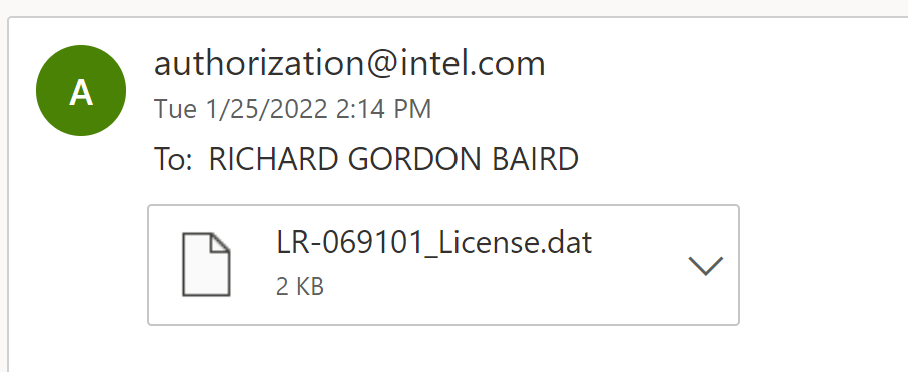
\includegraphics[scale=.8]{figures/licensedat.png}
        \caption{Save the .dat file to a safe location}
        \label{fig:my_label}
    \end{figure}
\end{frame}
\begin{frame}{License Installation}
   Once saved go back to the computer properties dialog from slide 7. On the right side -- or bottom if the dialog isn't expanded -- find and select \quotes{advanced System Settings}.
   \begin{figure}
       \centering
       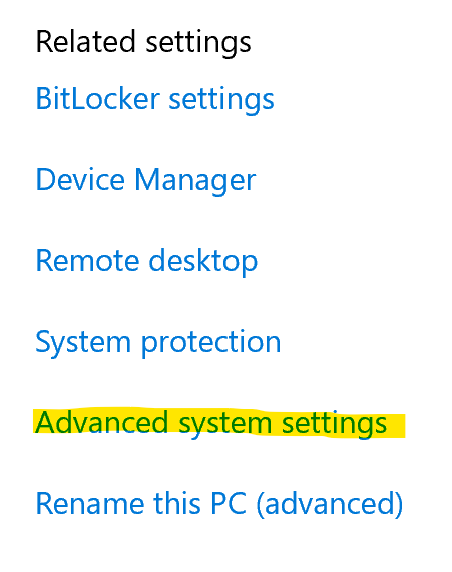
\includegraphics[scale=.5]{figures/advancedsettings.png}
       \caption{Advanced System Settings}
       \label{fig:my_label}
   \end{figure}
\end{frame}
\begin{frame}{License Installation}
    From here Select \quotes{Environment Variables} $\longrightarrow$ \quotes{User Variables} $\longrightarrow$ \quotes{New}\par
    From here add the variable name \quotes{LM\_LICENSE\_FILE}. Set as the value the path to the .dat file downloaded earlier. Press Okay and Okay and close the system properties. See the next slide for a visual guide.
\end{frame}
\begin{frame}{License Installation}
    \begin{figure}
        \centering
        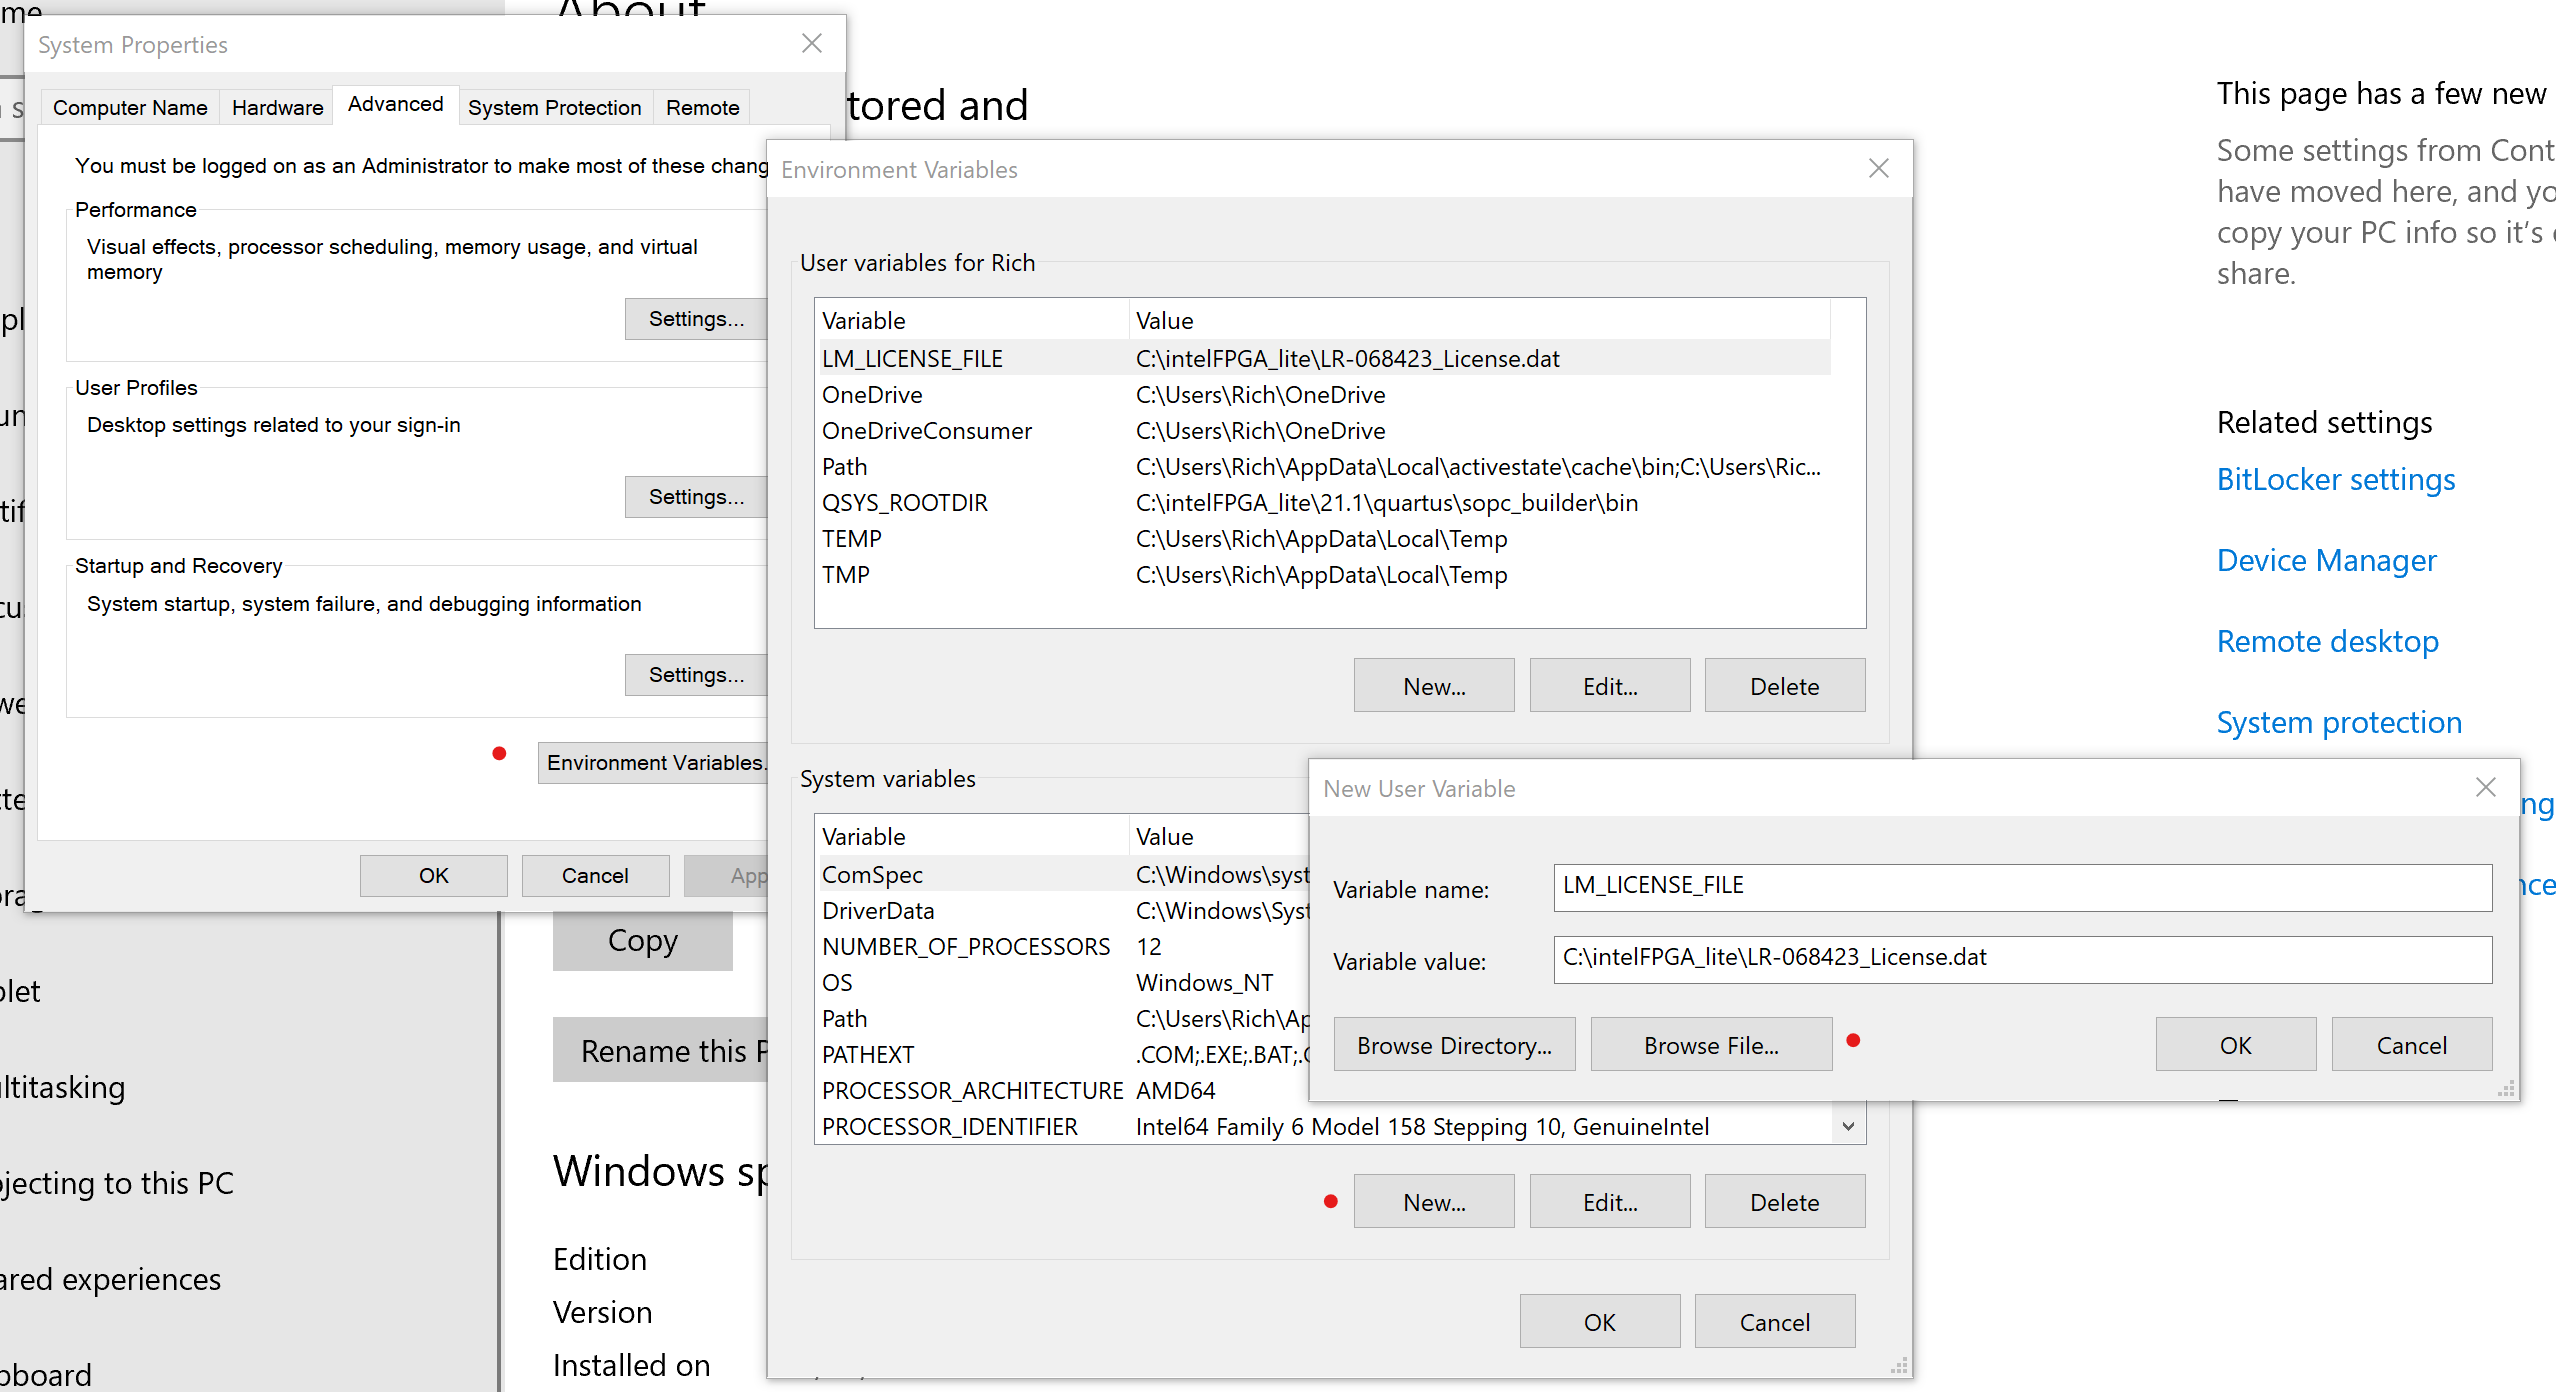
\includegraphics[height=16em]{figures/envvars.png}
        \caption{Add environment variable}
        \label{fig:my_label}
    \end{figure}
\end{frame}
\subsection{Connect Questa and Quartus}
\begin{frame}{Quartus Setup}
    Launch Quartus and go to tools $\longrightarrow$ options $\longrightarrow$ EDA Tool Options $\longrightarrow$ Questa Intel FPGA\par
    Type the location of the Questa executable in the space provided. On windows the default location is C:\textbackslash{}intelFPGA\textbackslash{}21.1\textbackslash{}questa\_fse\textbackslash{}win64
    \begin{multicols}{2}
        \begin{figure}
        \centering
        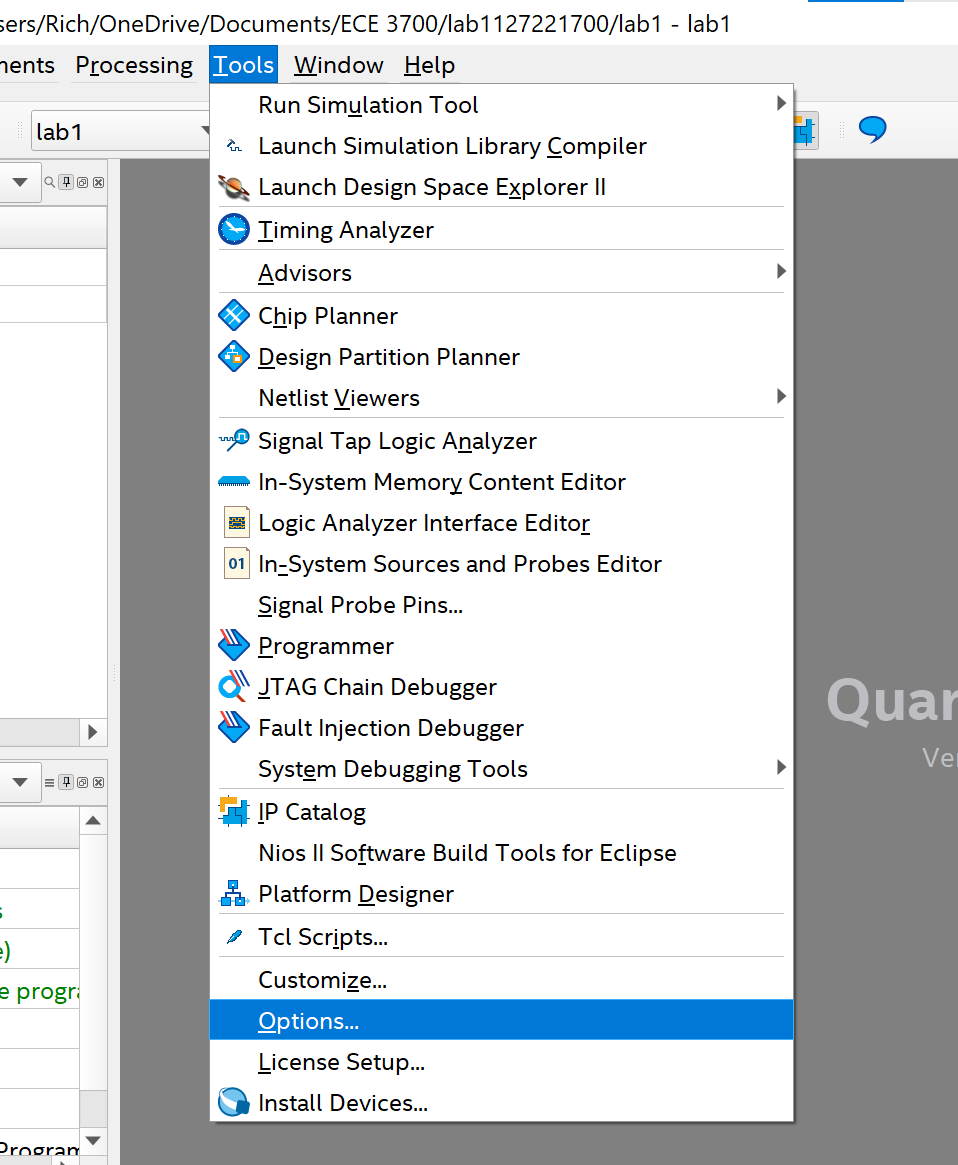
\includegraphics[scale=.3]{figures/quartusopts.png}
        \label{fig:my_label}
    \end{figure}
    \begin{figure}
        \centering
        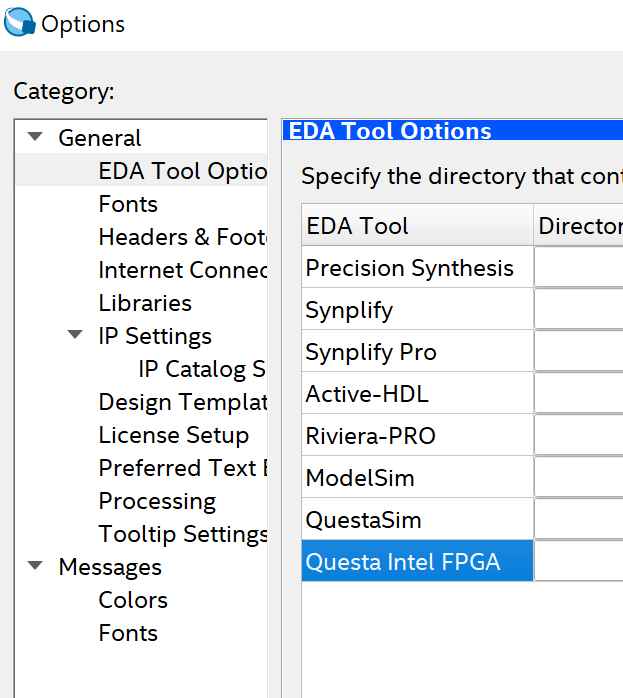
\includegraphics[scale=.5]{figures/edatool.png}
        \label{fig:my_label}
    \end{figure}
    \end{multicols}
\end{frame}
\begin{frame}{Quartus Setup}
    Go to Assignments $\longrightarrow$ Settings $\longrightarrow$ EDA Tool Settings $\longrightarrow$ Simulation\par
    Select the \quotes{Tool name:} drop down and choose \quotes{Questa Intel FPGA} and press okay.
    \begin{figure}
        \centering
        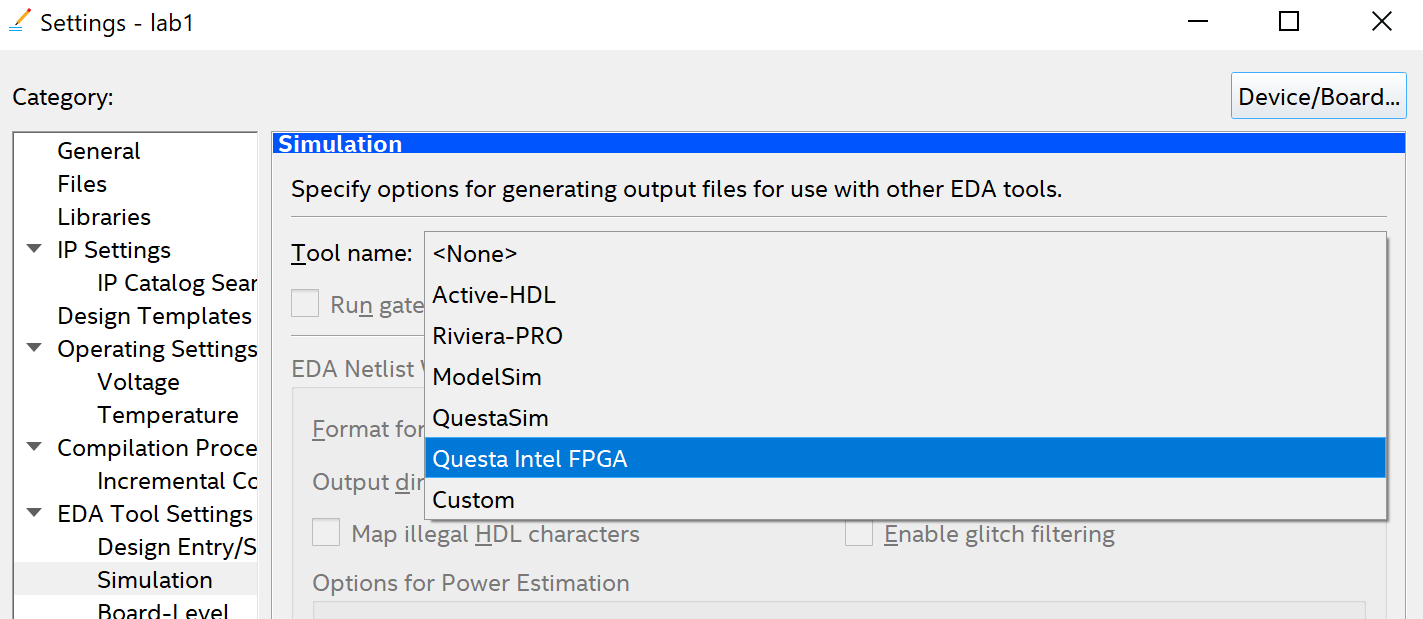
\includegraphics[scale=.5]{figures/simtool.png}
        \label{fig:my_label}
    \end{figure}
\end{frame}
\end{document}